\documentclass[aspectratio=169, 10pt]{beamer}

\usepackage{bm} % bold math
\usepackage{fontspec}
\usepackage{minted}
\usepackage{pgf-pie}
\usepackage{tikz}

% Custom commands and environments
\makeatletter
\newcommand\version[1]{\renewcommand\@version{#1}}
\newcommand\@version{}
\def\insertversion{\@version}

\newcommand\course[1]{\renewcommand\@course{#1}}
\newcommand\@course{}
\def\insertcourse{\@course}

\newcommand\coursetitle[1]{\renewcommand\@coursetitle{#1}}
\newcommand\@coursetitle{}
\def\insertcoursetitle{\@coursetitle}

\newcommand\lecturenumber[1]{\renewcommand\@lecturenumber{#1}}
\newcommand\@lecturenumber{}
\def\insertlecturenumber{\@lecturenumber}
\makeatother

\newcommand{\slidetitle}[1]{{\xbseries \large \structure{#1}} \bigskip}
\newcommand{\term}[1]{{\color{blue} #1}}
\newcommand{\leftspace}{\hspace{1em}}
\newcommand{\inlinearrow}{
  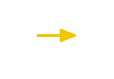
\begin{tikzpicture}[baseline]
    \node [anchor=base] (x) {};
    \draw [rawarrow] (x.mid west) -- ($(x.mid west) + (2em,0)$);
  \end{tikzpicture}
}

\newenvironment{slide}
{\begin{frame}[fragile,environment=slide]\vskip0pt plus 1filll}
{\vskip0pt plus 1filll\end{frame}}

% LaTeX

\setlength{\leftmargini}{1em}

% Common Information

\author{Jon Eyolfson}
\course{ECE 353}
\coursetitle{Systems Software}
\date{2024 Winter}

% fontspec

\defaultfontfeatures{Ligatures=TeX}
% \setmainfont{Domine}
\setsansfont{Inter}[
  FontFace={ul}{n}{Font=*-Thin},
  FontFace={el}{n}{Font=*-ExtraLight},
  FontFace={l}{n}{Font=*-Light},
  FontFace={sb}{n}{Font=*-SemiBold},
  FontFace={eb}{n}{Font=*-ExtraBold},
  FontFace={xb}{n}{Font=*-Black},
]
\setmonofont[Contextuals=AlternateOff, Ligatures=TeXOff]{Iosevka}[
  FontFace={xb}{n}{Font=*-Heavy},
]

%% Font Weights

\DeclareRobustCommand{\ulseries}{\fontseries{ul}\selectfont}
\DeclareTextFontCommand{\textul}{\ulseries}
\DeclareRobustCommand{\elseries}{\fontseries{el}\selectfont}
\DeclareTextFontCommand{\textel}{\elseries}
\DeclareRobustCommand{\lseries}{\fontseries{l}\selectfont}
\DeclareTextFontCommand{\textl}{\lseries}
\DeclareRobustCommand{\sbseries}{\fontseries{sb}\selectfont}
\DeclareTextFontCommand{\textsb}{\sbseries}
\DeclareRobustCommand{\ebseries}{\fontseries{eb}\selectfont}
\DeclareTextFontCommand{\texteb}{\ebseries}
\DeclareRobustCommand{\xbseries}{\fontseries{xb}\selectfont}
\DeclareTextFontCommand{\textxb}{\xbseries}

% tikz

\usetikzlibrary{
  arrows,
  arrows.meta,
  automata,
  backgrounds,
  calc,
  decorations.pathreplacing,
  matrix,
  positioning,
  overlay-beamer-styles,
  shapes,
  shapes.multipart,
  tikzmark,
}

\tikzstyle{rawarrow} = [
  -{Latex[round]},
  line width=1pt,
  yellow,
  shorten >=3pt,
  shorten <=3pt,
  font=\small,
  text=black,
]

\tikzstyle{arrow} = [
  -{Latex[round]},
  line width=1pt,
  yellow,
  shorten >=3pt,
  shorten <=3pt,
  transform canvas={yshift=3pt},
  font=\small,
  text=black,
]

\newcommand{\tikzmarkcoord}[1]{([yshift=3pt]pic cs:#1)}

% minted

\setminted{style=eyolfson, fontsize=\small, escapeinside=||}
\setmintedinline{fontsize=\normalsize}

% hyperref

\hypersetup{colorlinks, urlcolor=blue}

% beamer
\setbeamersize{text margin left=16mm, text margin right=16mm}
\setbeamertemplate{itemize items}[circle]
\setbeamercolor{item}{fg=black}
\setbeamercolor{structure}{fg=darkblue}
\setbeamerfont{frametitle}{series=\bfseries, parent=structure}
\setbeamertemplate{navigation symbols}{}
\setbeamertemplate{headline}{}
\setbeamertemplate{footline}{
  \begin{tikzpicture}[
    remember picture,
    overlay,
    shift={(current page.south west)},
  ]
    \path [fill=gray] (144mm, 0) -- (160mm, 16mm) -- (160mm, 0);
    \node [inner sep=3.5mm, outer sep=0, text=black, anchor=base east,
           align=right, yshift=3.5mm]
          at (current page.south east) {\ttfamily \small \insertframenumber{}};
  \end{tikzpicture}
}
\setbeamertemplate{title page}{
  \begin{tikzpicture}[
    remember picture,
    overlay,
    shift={(current page.south west)},
    background rectangle/.style={fill=darkblue},
    show background rectangle,
  ]
    \node [anchor=center, align=center, text=white, text width=40mm, scale=3.2]
          at (\paperwidth / 2, \paperheight * 2 / 3)
          {\xbseries \inserttitle{}};
    \node [anchor=base west, align=left, inner sep=0, text=white, yshift=2.5mm]
          at (16mm, \paperheight / 3)
          {\insertdate{} \insertcourse{}: \insertcoursetitle{}};
    \node [anchor=base west, align=left, inner sep=0, text=white, yshift=-2.5mm]
          at (16mm, \paperheight / 3)
          {\insertauthor};
    \node [anchor=base east, align=right, inner sep=0, text=white, yshift=2.5mm]
          at (144mm, \paperheight / 3)
          {Lecture \insertlecturenumber{}};
    \node [anchor=base east, align=right, inner sep=0, text=white,
           yshift=-2.5mm]
          at (144mm, \paperheight / 3)
          {\ttfamily \insertversion{}};
    \node [align=center, anchor=south, inner sep=0, text=white, yshift=3.5mm]
          (license) at (\paperwidth / 2, 0)
          {\fontsize{7pt}{7pt}\selectfont This  work is licensed under a
           \href{http://creativecommons.org/licenses/by-sa/4.0/}
                {\color{lightblue} Creative Commons Attribution-ShareAlike 4.0
                 International License}};
  \end{tikzpicture}
}

% xcolor

%% Primary Colour

\definecolor{pantone655}{RGB}{0, 42, 92} % #002a5c
\colorlet{darkblue}{pantone655}

%% Secondary Colours

\definecolor{pantone633}{RGB}{0, 139, 176} % #008bb0
\colorlet{blue}{pantone633}

\definecolor{pantonewarmred}{RGB}{220, 70, 51} % #dc4633
\colorlet{red}{pantonewarmred}

\definecolor{pantone3285}{RGB}{0, 161, 137} % #00a189
\colorlet{cyan}{pantone3285}

\definecolor{pantone7722}{RGB}{13, 83, 77} % #0d534d
\colorlet{darkcyan}{pantone7722}

\definecolor{pantone376}{RGB}{141, 191, 46} % #8dbf2e
\colorlet{green}{pantone376}

\definecolor{pantone2613}{RGB}{109, 36, 122} % #6d247a
\colorlet{violet}{pantone2613}

\definecolor{pantone2985}{RGB}{111, 199, 234} % #6fc7ea
\colorlet{lightblue}{pantone2985}

\definecolor{pantone227}{RGB}{171, 19, 104} % #ab1368
\colorlet{magenta}{pantone227}

\definecolor{pantone7406}{RGB}{241, 197, 0} % #f1c500
\colorlet{yellow}{pantone7406}

%% Neutrals

\definecolor{pantonecoolgray2}{RGB}{208, 209, 201} % #d0d1c9
\colorlet{gray}{pantonecoolgray2}


\title{Midterm Review}
\lecturenumber{18}
\version{2.0.0}

\begin{document}
  \begin{frame}[plain, noframenumbering]
    \titlepage
  \end{frame}

  \begin{slide}
    \slidetitle{There are 3 Major Concepts in This Course}

    You'll learn how the following applies to operating systems:
    \begin{itemize}
      \item Virtualization
      \item Concurrency
      \item Persistence
    \end{itemize}
  \end{slide}

  \begin{slide}
    \slidetitle{Kernel Interfaces Operate Between CPU Mode Boundaries}

    The lessons from the lecture:
    \begin{itemize}
      \item Code running in kernel mode is part of your kernel
      \item System calls are the interface between user and kernel mode
        \begin{itemize}
          \item Every program must use this interface!
        \end{itemize}
      \item File format and instructions to define a simple ``Hello world''
            (in 168 bytes)
        \begin{itemize}
          \item Difference between API and ABI
          \item How to explore system calls
        \end{itemize}
      \item Different kernel architectures shift how much code runs in kernel
            mode
    \end{itemize}
  \end{slide}

  \begin{slide}
    \slidetitle{Operating Systems Provide the Foundation for Libraries}

    We learned:
    \begin{itemize}
      \item Dynamic libraries and a comparison to static libraries
      \begin{itemize}
        \item How to manipulate the dynamic loader
      \end{itemize}
      \item Example of issues from ABI changes without API changes
    \end{itemize}

  \end{slide}

  \begin{slide}

    \slidetitle{Unix Systems Clone Processes with a Parent/Child Relationship}

    \begin{itemize}
      \item You can only create new processes with \texttt{fork}
      \item After a \texttt{fork} both processes are exactly the same
      \begin{itemize}
        \item except for the value of \texttt{pid} (the child is always 0)
      \end{itemize}
      \item The scheduler decides when to run either process
    \end{itemize}

  \end{slide}

  \begin{slide}

    \slidetitle{You're Responsible for Managing Processes}

    The operating system maintains a strict parent/child relationship
    \bigskip
    
    You should be able to identify (and prevent) the following:
    \begin{itemize}
      \item Zombie processes
      \item Orphan processes
    \end{itemize}

  \end{slide}

  \begin{slide}
    \slidetitle{We Explored Basic IPC in an Operating System}

    Some basic IPC includes:
    \begin{itemize}
      \item \texttt{read} and \texttt{write} through file descriptors (could be a regular file)
      \item Redirecting file descriptors for communcation
      \item Signals
    \end{itemize}
    \bigskip

    Signals are like interrupts for user processes

    \leftspace{}The kernel has to handle all 3 kinds of ``interrupts''
  \end{slide}

  \begin{slide}

    \slidetitle{Scheduling Involves Trade-Offs}

    We looked at few different algorithms:

    \begin{itemize}
      \item First Come First Served (FCFS) is the most basic scheduling algorithm
      \item Shortest Job First (SJF) is a tweak that reduces waiting time
      \item Shortest Remaining Time First (SRTF) uses SJF ideas with preemptions
      \item SRTF optimizes lowest waiting time (or turnaround time)
      \item Round-robin (RR) optimizes fairness and response time
    \end{itemize}

  \end{slide}

  \begin{slide}

    \slidetitle{Scheduling Gets Even More Complex}

    There are more solutions, and more issues:

    \begin{itemize}
      \item Introducing priority also introduces priority inversion
      \item Some processes need good interactivity, others not so much
      \item Multiprocessors may require per-CPU queues
      \item Real-time requires predictability
      \item Completely Fair Scheduler (CFS) tries to model the ideal fairness
    \end{itemize}

  \end{slide}

  \begin{slide}

    \slidetitle{Page Tables Translate Virtual to Physical Addresses}

    The MMU is the hardware that uses page tables, which may:
    \begin{itemize}
      \item Be a single large table (wasteful, even for 32-bit machines)
      \item Use the kernel allocated pages from a free list
      \item Be a multi-level to save space for sparse allocations
      \item Use a TLB to speed up memory accesses
    \end{itemize}

  \end{slide}

  \begin{slide}

    \slidetitle{Threads Enable Concurrency}

    We explored threads, and related them to something we already know (processes)
    \begin{itemize}
      \item Threads are lighter weight, and share memory by default
      \item Each process can have multiple threads (but just one at the start)
    \end{itemize}

  \end{slide}

  \begin{slide}

    \slidetitle{Both Processes and (Kernel) Threads Enable Parallelization}

    \begin{itemize}
      \item Each process can have multiple (kernel) threads
      \item Most implementations use one-to-one user-to-kernel thread mapping
      \item The operating system has to manage what happens during a fork, or signals
      \item We now have synchronization issues
    \end{itemize}

  \end{slide}

  \begin{slide}

    \slidetitle{A Forking Question}

    Consider the following code:

    \begin{minted}{c}
int main() {
  pid_t first = fork();
  pid_t second = fork();
  pid_t third = fork();
  printf("first=%d second=%d third=%d\n", first, second, third);
}
    \end{minted}
    \vspace{1em}

    What is one reasonable set of outputs (assume the initial process is pid 2)?
    \medskip

    Are the outputs in any specific order?
    \medskip

    What do the relationships between processes look like?

  \end{slide}

  \begin{slide}
    
    \slidetitle{Example Midterms}

    This is the style of midterm I typically write:

    \small
    \url{https://eyolfson.com/media/courses/utoronto/ece344/2023-fall/midterm.pdf}

    \url{https://eyolfson.com/media/courses/utoronto/ece353/2023-winter/midterm.pdf}

    \url{https://eyolfson.com/media/courses/ucla/cs111/21fall/midterm.pdf}

  \end{slide}

\end{document}
